\documentclass[main.tex]{subfiles}
\begin{document}
\begin{enumerate}

\subsection*{Section 1 Computer Architecture and High-Performance Computing}

\item [1.] \textbf{Q.} After graduating, you are asked to become the lead computer designer at New Computers Inc. You have invented a scheme that reduces the loads and stores normally associated with procedure calls and returns. The first thing you do is run some experiments with and without this optimization. Your experiments use the same state-of-the-art optimizing compiler that will be used with either version of the computer. These experiment reveal the following information:
\begin{itemize}
    \item The clock rate of the un-optimized version is 15\% higher.
    \item 45\% of the instructions in the un-optimized version are loads and stores.
    \item The optimized version executes one-third as many loads and stores as the un-optimized version.
    \item For all other instructions the dynamic execution counts are unchanged.
    \item All instructions (including load and store) take one clock cycle.
\end{itemize}
Which is faster? The optimized version or the un-optimized one. Justify your decision quantitatively by computing an improvement factor to validate your answer. 

\textbf{A.} Compiler performance can be quantified by execution time $T$ (Eq. \ref{eq:executionTime}) where $IC$ is the instruction count in a given program, $CPI$ is number of cycles per instruction, and $CT$ is the clock time. Additionally $CT=1/f$ where $f$ is the clock rate.

\begin{equation} \label{eq:executionTime}
T = IC \times CPI \times CT
\end{equation}

The un-optimized compilers clock rate is 15\% higher than the optimized version $\therefore f_{u} = 1.15f_{o}$. The cycle time for the optimized compiler is $\therefore CT_o = 1.15CT_u$. The un-optimized compiler instructions are comprised of 45\% loads and stores and the optimized compiler instructions, which is 1/3 of the un-optimized, are comprised of 15\% loads and stores. However since it is given that all instructions, including load and store, take one clock cycle the percent of loads and stores is irrelevant and $\therefore CPI_o = CPI_u$. For the same program the instruction count for the optimized and un-optimized compilers will remain the same $\therefore IC_o = IC_u$. Clock time is the only factor the differs between compilers and $\because CT_o > CT_u \therefore T_o > T_u$. An increase in execution time for the optimized compiler is a degradation in performance and therefore the un-optimized compiler is the faster version.

\item [2.] The IEEE 754 Floating point number standard format for single precision floating-point numbers can be summarized as follows. The 32 bits number is divided as shown in figure \ref{fig:f1}. A number is normalized if the exponent value is between 1 and 254, and is denormalized if the exponent value is 0 and the fraction value is not 0. The value of a normalized number is $(-1)^S \times (1+Fraction) \times 2^{(Exponent-bias)}$ and the value of a denormalized number is $(-1)^S \times (0+Fraction) \times 2^{(1-bias)}$. Where the bias value is 127. Please answer the following questions:

\begin{figure}
\centering\fbox{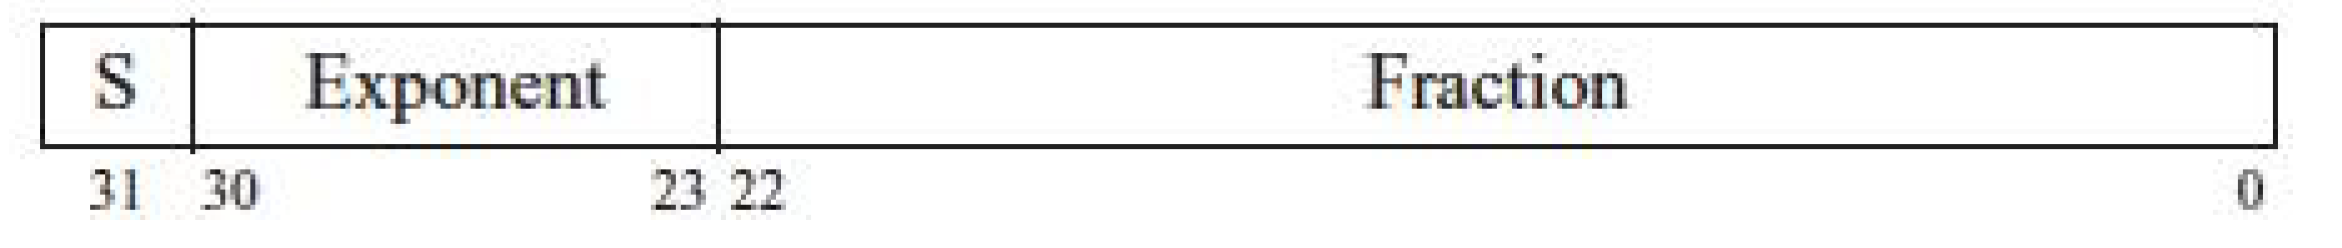
\includegraphics[width=4.0in]{2018spring/figures/02q_a.png}}
\caption{32 bits number}
\label{fig:f1}
\end{figure}

\begin{enumerate}
    \item \textbf{Q.} What are the maximum and minimum normalized numbers that can be computed using single precision format? \textbf{A.} The maximum normalized number that can be computed using single bit precision is comprised of the sign bit $b_{31} = 0$ with $S=0$, exponent bits $b_{30} b_{29} \cdots b_{24}$ set to 1 and $b_{23}$ set to 0, accounting for the exponent bit values of all zeros and all ones reserved for special numbers, with the $Exponent = \sum_{i=0}^{7} b_{23+i} 2^{+i} = 254$, and fraction bits $b_{22} b_{21} \cdots b_{0}$ set to 1 with the $Fraction = \sum_{i=1}^{23} b_{23-i} 2^{-i} \approx 0.999$, resulting in the calculation $(-1)^0 \times (1+0.999) \times 2^{(254-127)} = 1 \times 1.999 \times \num{1.7014118e38} \approx \num{3.401e38}$. The absolute minimum normalized number that can be computed using single bit precision is comprised of the sign bit $b_{31} = 1$ with $S=1$, $Exponent$ and $Fraction$ that same as for the maximum calculation, and calculated as $(-1)^1 \times (1+0.999) \times 2^{(254-127)} = -1 \times 1.999 \times \num{1.701e38} \approx \num{-3.401e38}$.
    
    \item \textbf{Q.} What are the maximum and minimum denormalized numbers that can be computed using single precision format? \texbf{A.} The (absolute) maximum denormalized single bit precision number is comprised of sign bit $b_{31} = 0$ or $b_{31} = 1$, exponent bits $b_{30} b_{29} \cdots b_{23}$ set to 0, and fraction bits $b_{22} b_{21} \cdots b_{0}$ set to 1 with value $\sum_{i=1}^{23} b_{23-i} 2^{-i} = (1-2^{-23})$, resulting in a calculated value (positive example) of $(-1)^0 \times (0+(1-2^{-23}) \times 2^{(1-127)} \approx \pm\num{1.18e-38}$. The absolute minimum denormalized single bit precision number differs from the maximum with fraction bits $b_{22} b_{21} \cdots b_{1}$ set to 0 and $b_{0}$ set to 1 with value $\sum_{i=1}^{23} b_{23-i} 2^{-i} = 2^{-23}$ resulting in a calculated value (positive example) of $(-1)^0 \times 0+2^{-23} \times 2^{(1-127)} \approx \pm\num{1.4e-45}$.
    
    \item \texbt{Q.} If we change the Exponent size to be 10 bits instead of 8 and the fraction to be 21 bits instead of 23 bits:
    
    \begin{enumerate}
        \item \textbf{Q.} What should the bias value be? \textbf{A.} The original bias of 127 is half the maximum exponent value of 254, using that logic the new bias should equal $\frac{2^{10} - 2}{2} = \frac{1022}{2}=512$
        
        \item \textbf{Q.} Repeat question 2 (wording confusing assume 2a) for the new format. \textbf{A.} The absolute maximum normalized single bit precision number is comprised of sign bit $b_{31} = 0$ (positive example), exponent bits $b_{30} b_{29} \cdots b_{22}$ set to 1 and $b_{21}$ set to 0, accounting for all ones reserved for positive and negative infinity, with value $\sum_{i=0}^{9} b_{21+i} 2^{+i} = 1022$, and fraction bits $b_{20} b_{19} \cdots b_{0}$ set to 1 with value $\sum_{i=1}^{21} b_{21-i} 2^{-i} = (1-2^{-21})$, resulting in the calculation $(-1)^0 \times (1+1-2^{-21}) \times 2^{(1022-512)} \approx \pm \num{6.7e153}$. The absolute minimum normalized number that can be computed using single bit precision is comprised of the sign bit $b_{31} = 1$ (positive example), exponent bits $b_{30} b_{29} \cdots b_{22}$ set to 0 and $b_{21}$ set to 1 with exponent value $\sum_{i=0}^{9} b_{21+i} 2^{+i} = 1$, and fraction bits $b_{20} b_{19} \cdots b_{0}$ set to 0 with fraction value $\sum_{i=1}^{21} b_{21-i} 2^{-i} = 0$, resulting in the calculation  $(-1)^1 \times (1+0) \times 2^{(1-512)} \approx \pm \num{1.49e-154}$.
        
        \item \textbf{Q.} Repeat question 3 (wording confusing assume 2b) for the new format. \textbf{A.} The absolute maximum denormalized single bit precision number is comprised of sign bit $b_{31} = 0$ (positive example), exponent bits $b_{30} b_{29} \cdots b_{21}$ set to 0, and fraction bits $b_{20} b_{19} \cdots b_{0}$ set to 1 with fraction value $\sum_{i=1}^{21} b_{21-i} 2^{-i} = (1-2^{-21})$, resulting in a calculated value (positive example) of $(-1)^0 \times (0+(1-2^{-21})) \times 2^{(1-512)} \approx \pm\num{1.49e-154}$. The absolute minimum denormalized single bit precision number differs from the maximum with fraction bits $b_{20} b_{19} \cdots b_{1}$ set to 0 and $b_{0}$ set to 1 with fractional value $\sum_{i=1}^{21} b_{21-i} 2^{-i} = 2^{-21}$ resulting in a calculated value (positive example) of $(-1)^0 \times 0+2^{-21} \times 2^{(1-512)} \approx \pm\num{7.11e-161}$.
    
    \end{enumerate}
    
    \item \textbf{Q.} Represent the following two decimal numbers in Single Precision format:
    
    \begin{enumerate}
        \item \textbf{Q.} 0.1 \textbf{A.} Multiply the decimal fraction by 2, take the integer component, and repeat with the new fraction until a fraction of zero is found or the precision limit of 23 fraction digits is reached. Decimal 0.1 cannot be represented in single precision format exactly, only approximated.
        
        \medskip
        
        \begin{itemize}[label={}]
            \item $0.1 \times 2 = 0.2 = 0 + 0.2 \Rightarrow b_{22}=0$
            \item $0.2 \times 2 = 0.4 = 0 + 0.4 \Rightarrow b_{21}=0$
            \item $0.4 \times 2 = 0.8 = 0 + 0.8 \Rightarrow b_{20}=0$
            \item $0.8 \times 2 = 1.6 = 1 + 0.6 \Rightarrow b_{19}=1$
            \item $0.6 \times 2 = 1.2 = 1 + 0.2 \Rightarrow b_{18}=1$
            \item $\cdots$
            \item $0.2 \times 2 = 0.4 = 0 + 0.4 \Rightarrow b_{5}=0$
            \item $0.4 \times 2 = 0.8 = 0 + 0.8 \Rightarrow b_{4}=0$
            \item $0.8 \times 2 = 1.6 = 1 + 0.6 \Rightarrow b_{3}=1$
            \item $0.6 \times 2 = 1.2 = 1 + 0.2 \Rightarrow b_{2}=1$
            \item $0.2 \times 2 = 0.4 = 0 + 0.4 \Rightarrow b_{1}=0$
            \item $0.4 \times 2 = 0.8 = 0 + 0.8 \Rightarrow b_{0}=0$
        \end{itemize}
        
        \medskip

        $$
        \begin{aligned}
        (0.1)_{10} &\approx (0.00011001100110011001100)_2\\
        &= (1.1001100110011001100)_2 \times 2^{-4}
        \end{aligned}
        $$
        
        \medskip
        
        \begin{itemize}[label={}]
            \item sign bit: $b_{31}=(0)_2$
            \item exponent: $-4$ biased as $(127+(-4))_{10} = (123)_{10} = (01111011)_2$
            \item fraction: $(1001100110011001100)_2$
        \end{itemize}
        
        \medskip
        
        decimal $(0.1)_{10}$ $\Rightarrow$ single precision $(0$ $01111011$ $10011001100110011001101)_{2}$ 
        
        \medskip
        
        The final 1101 adds additional precision after the 4 digit normalization shift.
        
        \item \textbf{Q.} 33554431 \textbf{A.} Iteratively divide 33554431 by 2 noting the quotient and remainder until a quotient of 0 is reached.\\ 
        
        \begin{center}
        \begin{tabular}{ |c c c| } 
            \hline
            Division & Quotient & Remainder\\  
            \hline\hline
            33554431/2 & 16777215 & 1 \\ 
            \hline
            16777215/2 & 8388607 & 1 \\ 
            \hline
            8388607/2 & 4194303 & 1 \\ 
            \hline
            4194303/2 & 2097151 & 1 \\ 
            \hline
            2097151/2 & 1048575 & 1 \\ 
            \hline
            1048575/2 & 524287 & 1 \\ 
            \hline
            524287/2 & 262143 & 1 \\ 
            \hline
            262143/2 & 131071 & 1 \\ 
            \hline
            131071/2 & 65535 & 1 \\ 
            \hline
            65535/2 & 32767 & 1 \\ 
            \hline
            32767/2 & 16383 & 1 \\ 
            \hline
            16383/2 & 8191 & 1 \\ 
            \hline
            8191/2 & 4095 & 1 \\ 
            \hline
            4095/2 & 2047 & 1 \\ 
            \hline
            2047/2 & 1023 & 1 \\ 
            \hline
            1023/2 & 511 & 1 \\ 
            \hline
            511/2 & 255 & 1 \\ 
            \hline
            255/2 & 127 & 1 \\ 
            \hline
            127/2 & 63 & 1 \\ 
            \hline
            63/2 & 31 & 1 \\ 
            \hline
            31/2 & 15 & 1 \\ 
            \hline
            15/2 & 7 & 1 \\ 
            \hline
            7/2 & 3 & 1 \\ 
            \hline
            3/2 & 1 & 1 \\ 
            \hline
            1/2 & 0 & 1 \\ 
            \hline
        \end{tabular}
        \end{center}
        
        \medskip
        
        Read the 25 bits from the bottom (Most Significant Bit) to top (Least Significant Bit), and normalize the binary value 
        
        $$
        (1.111111111111111111111111 \times 2^{24})_2.
        $$
        
        When dealing with the positive whole number $33554431$ the value to the right of the decimal point is zero and the sign bit $b_{31} = 0$. Calculate the exponent bits $b_{30} b_{29} \cdots b_{23}$ with a bias of 127 and an exponent decimal value of $127+24=151$.
        
        \medskip
        
        \begin{center}
        \begin{tabular}{ |c c c| } 
            \hline
            Division & Quotient & Remainder\\  
            \hline\hline
            151/2 & 75 & 1 \\ 
            \hline
            75/2 & 37 & 1 \\ 
            \hline
            37/2 & 18 & 1 \\ 
            \hline
            18/2 & 9 & 0 \\ 
            \hline
            9/2 & 4 & 1 \\ 
            \hline
            4/2 & 2 & 0 \\ 
            \hline
            2/2 & 1 & 0 \\ 
            \hline
            1/2 & 0 & 1 \\ 
            \hline
        \end{tabular}
        \end{center}
        
        \medskip
        
        Read the 8 bits from the bottom (Most Significant Bit) to top (Least Significant Bit) where $b_{30}b_{29} \cdots b_{23} = (10010111)_2$ Determine the 23 bits of the mantissa (from left to right) from the right of the decimal point where $b_{22}b_{21} \cdots b_{0} = (11111111111111111111111)_{2}$. However we still have a remaining $1$. Compile the sign bit $b_{31}$, exponent bits $b_{30}b_{29} \cdots b_{23}$, and mantissa bits $b_{22}b_{21} \cdots b_{0}$ into IEEE 754 floating point single precision format where $(33554431)_{10} =$ $(0$ $10010111$ $11111111111111111111111)_2$ 
    \end{enumerate}
    
    \item \textbf{Q.} Take the values you computed in (d) and convert them back into decimal. Did the numbers change? Explain why. \textbf{A.} 

    \begin{enumerate}
        \item $(0$ $01111011$ $10011001100110011001101)_2$ contains the sign bit $b_{31} = 0$, the decimal value of the exponent bits $b_{23}*2^0 + b_{24}*2^1 + \cdots + b_{30}*2^7 = 1*2^0 + 1*2^1 + \cdots + 0*2^7 = 123$, and the decimal value of the mantissa bits $b_{22}*2^{-1} + b_{21}*2^{-2} + \cdots + b_{0}*2^{-23} = 1*2^{-1} + 0*2^{-2} + \cdots + 1*2^{-23} = 0.6000015735626221$. Calculate the decimal value using 
        $(-1)^S \times (1+Fraction) \times 2^{(Exponent-bias)} = (-1)^0 \times (1+0.6000015735626221) \times 2^{(123-127)} = 1.6000015735626221 \times 0.0625 = 0.10000009834766388125$. Decimal 0.1 cannot be represented in single precision format exactly (or any precision format), only approximated up to the maximum number of bits available in the mantissa, because as we can see in table # ... a loop of repeating values forms when multiplying the decimal by 2.
        
        \item $(0$ $10011000$ $00000000000000000000000)_2$ contains the sign bit $b_{31} = 0$, the exponent bits $b_{23}*2^0 + b_{24}*2^1 + \cdots + b_{30}*2^7 = 0*2^0 + 0*2^1 + \cdots + 1*2^7 = 152$, andd the mantissa bits $b_{22}*2^{-1} + b_{21}*2^{-2} + \cdots + b_{0}*2^{-23} = 0*2^{-1} + 0*2^{-2} + \cdots + 0*2^{-23} = 0$. Calculate the decimal value using 
        $(-1)^S \times (1+Fraction) \times 2^{(Exponent-bias)} = (-1)^0 \times (1+0) \times 2^{(152-127)} = 33554432$.
    \end{enumerate}
    
\end{enumerate}

\item [3.] \textbf{Q.} For a hypothetical CPU which has 64 bit virtual address and 41 bit physical address with two levels of cache. The L1 cache is virtually indexed and physically tagged. The L1 size is 8KB. The page size is 8KB. The L2 cache is 4MB. The block size is 64 bytes. Please illustrate the translation of virtual address to physical address, as well as the interactions to the TLB and L1/L2 Cache. Indicate how many bits are used for page number, page offset, TLB index, TLB tag, cache index, cache tag, etc. \\

    \textbf{A.} Figure \ref{fig:03_translation_general} illustrates the translation of a virtual address generated by the CPU to a physical address available in memory with the quantity of bits used enumerated in Table \ref{table:03_component_bit_count}. 
    
    \begin{figure}
    \centering\fbox{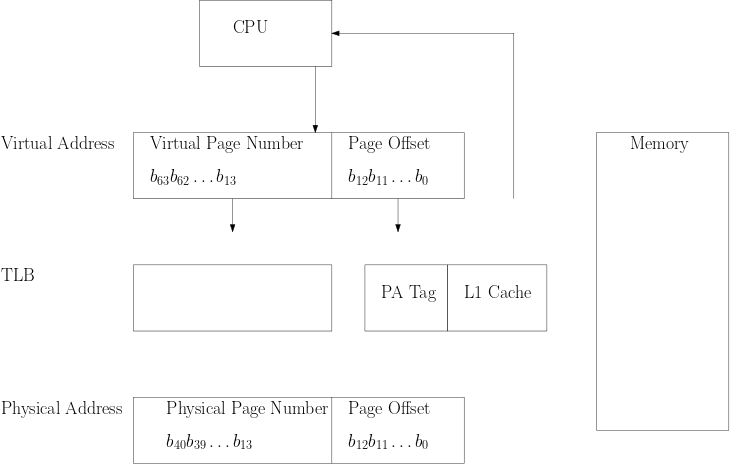
\includegraphics[width=6.0in]{2018spring/figures/03_translation.png}}
    \caption{In order to translate the virtual address generated by the CPU to a physical address available in the memory unit we utilize a page table, Translation Lookaside Buffer (TLB), Virtually Indexed Physically Tagged (VIPT) L1 cache, and an L2 cache. Use the given page size of $8\text{kB} = 8192 \text{ bits} = 2^{13}$  to determine the 13 bit page offset which is identical for the virtual and physical addresses. The 64 bit virtual address is composed of the 51 bit $\left(b_{63},b_{62},\dots,b_{13}\right)$ virtual page number and the 13 bit $\left(b_{12},b_{11},\dots,b_{0}\right)$ page offset. The 41 bit physical address is composed of the 28 bit $\left(b_{40},b_{39},\dots,b_{13}\right)$ physical page number and the 13 bit $\left(b_{12},b_{11},\dots,b_{0}\right)$ page offset. Use the given Virtually Indexed Physically Tagged (VIPT) 8KB L1 cache for the Translation Lookaside Buffer (TLB) for instructions (iTLB), and the 4MB L2 cache for the TLB for data (dTLB). Using a Virtually Indexed Physically Tagged (VIPT) 8KB L1 cache we can access the cache at the same time as the Translation Lookaside Buffer (TLB) but still get the protection of virtual memory.}
    \label{fig:03_translation_general}
    \end{figure}
    
    \begin{table}
    \centering
    \begin{tabular}{| c c |}
        \hline
        Component & Bit Count \\  
        \hline\hline
        virtual page number & 51\\
        \hline
        physical page number & 28 \\  
        \hline
        page offset & 13\\
        \hline
        TLB index & 0\\
        \hline
        TLB tag & 0\\
        \hline
        L1 cache index & 0\\
        \hline
        L1 cache tag & 0\\
        \hline
        L2 cache index & 0\\
        \hline
        L2 cache tag & 0\\
        \hline
    \end{tabular}
    \caption{Component Bit Count}
    \label{table:03_component_bit_count}
    \end{table}
\end{enumerate}
\end{document}